%%%%%%%%%%%%%%%%%%%%%%%%%%%%%%%%%%%%%%%%%%%%%%%%
\section{Background}


%%%%%%%%%%%%%%%%%%%%%%%%%%%%%%%%%%%%%%%%%%%%%%%%%%%
\begin{frame}

\frametitle{Pipeline}

Sequence of programs, running one after the other:
\begin{figure}
  \centering
  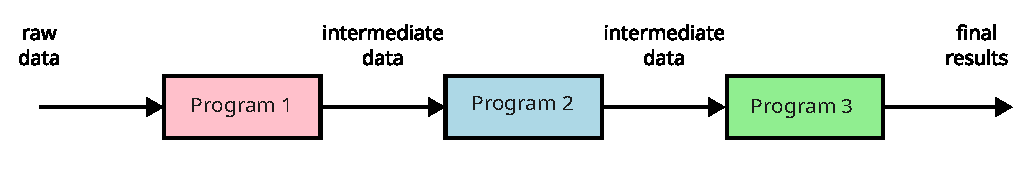
\includegraphics[width=\linewidth]{background/pipeline-example-straight.eps}
\end{figure}

\end{frame}


%%%%%%%%%%%%%%%%%%%%%%%%%%%%%%%%%%%%%%%%%%%%%%%%%%%
\begin{frame}

\frametitle{Pipeline}

Branching is also possible:
\begin{figure}
  \centering
  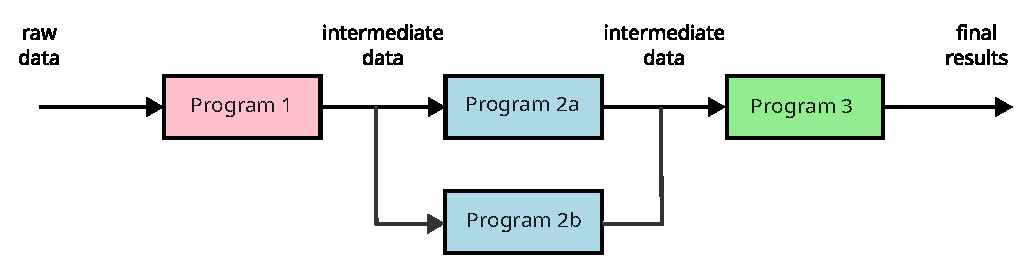
\includegraphics[width=\linewidth]{background/pipeline-example-branching.eps}
\end{figure}

\end{frame}


%%%%%%%%%%%%%%%%%%%%%%%%%%%%%%%%%%%%%%%%%%%%%%%%%%%
\begin{frame}

\frametitle{Counting characters}

Running a sequence of programs is not new to bioinformatics.
\vs

Suppose we wanted to count the number of words and characters in the first 1000 lines of the file {\texttt{alice29}}.
\vs

In Linux, we can do the following with a temporary file:
\begin{small}
\begin{table}
  \begin{tabular}{l}
  {\texttt{head -n 1000 alice29 {\textgreater}tmp1.txt}} \\
  {\texttt{wc -w -c tmp1.txt {\textgreater}alice29.count}} \\
  \end{tabular}
\end{table}
\end{small}
\vs

\pause

Or, we can use the vertical bar or ``pipe'' character (\textbar) as follows:
\begin{small}
\begin{table}
  \begin{tabular}{l}
  {\texttt{cat alice29 {\textbar} head -n 1000 {\textbar} wc -w -c {\textgreater}alice29.count}} \\
  \end{tabular}
\end{table}
\end{small}

\end{frame}


%%%%%%%%%%%%%%%%%%%%%%%%%%%%%%%%%%%%%%%%%%%%%%%%%%%
\begin{frame}

\frametitle{Make}

The program {\texttt{Make}} takes this one step further by allowing users to manage {\magenta{dependencies}}.
\vs

A file called {\texttt{Makefile}} is read by {\texttt{Make}}.
\vs

It can indicate that {\texttt{alice29.count}} is updated only if {\texttt{alice29}} was updated.

\end{frame}


%%%%%%%%%%%%%%%%%%%%%%%%%%%%%%%%%%%%%%%%%%%%%%%%%%%
\begin{frame}

\frametitle{Make}

\begin{figure}
  \centering
  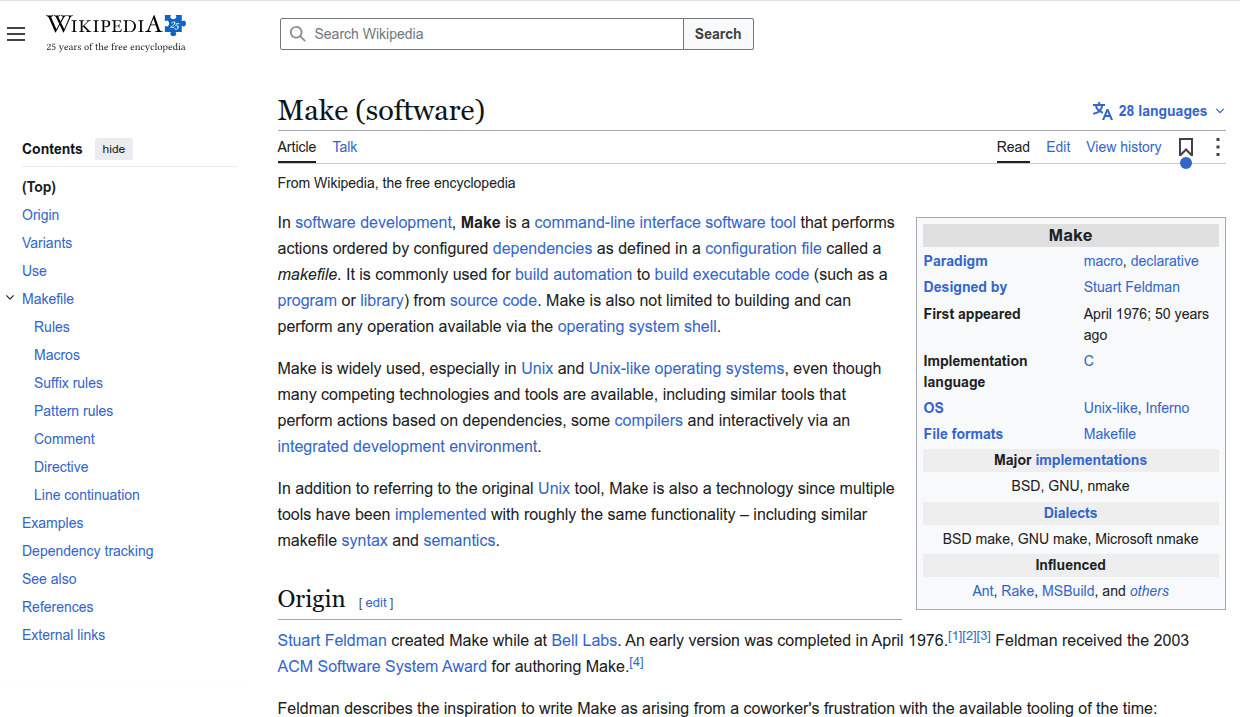
\includegraphics[width=\linewidth]{background/make-wikipedia}
\end{figure}

\end{frame}


%%%%%%%%%%%%%%%%%%%%%%%%%%%%%%%%%%%%%%%%%%%%%%%%%%%
\begin{frame}

\frametitle{Makefile}

Typically, a {\texttt{Makefile}} has a series of rules.  One rule looks like this:
\vs

\begin{figure}
  \centering
  {\fbox{
  \begin{tabular}{l}
\texttt{target:  prerequisites}\\
\texttt{{\D\D}command}\\
\texttt{{\D\D}$\vdots$}\\
\texttt{{\D\D}command}\\
  \end{tabular}
  }}
\end{figure}
\vs

{\red{$\rightarrow$}} If the dates of the files in the {\blue{prerequisites}} are newer than the {\green{target}}, then update the target by running the {\magenta{commands}} (which are preceded by a single tab character).

\end{frame}


%%%%%%%%%%%%%%%%%%%%%%%%%%%%%%%%%%%%%%%%%%%%%%%%%%%
\begin{frame}

\frametitle{``Make'' example}

As a series of commands:
\begin{scriptsize}
\begin{figure}
  \centering
  {\fbox{
  \begin{tabular}{l}
{\texttt{alice29.count:  alice29}} \\
{\D\D}{\texttt{head -n 1000 alice29 {\textgreater}tmp1.txt}} \\
{\D\D}{\texttt{wc -w -c tmp1.txt {\textgreater}alice29.count}} \\
  \end{tabular}
  }}
\end{figure}
\end{scriptsize}

\pause

As one long command with pipes:
\begin{scriptsize}
\begin{figure}
  \centering
  {\fbox{
  \begin{tabular}{l}
{\texttt{alice29.count:  alice29}} \\
{\D\D}{\texttt{cat alice29 {\textbar} head -n 1000 {\textbar} wc -w -c {\textgreater}alice29.count}} \\
  \end{tabular}
  }}
\end{figure}
\end{scriptsize}

\end{frame}


%%%%%%%%%%%%%%%%%%%%%%%%%%%%%%%%%%%%%%%%%%%%%%%%%%%
\begin{frame}

\frametitle{``Make'' example\footnote{V1}}

\begin{figure}
  \centering
  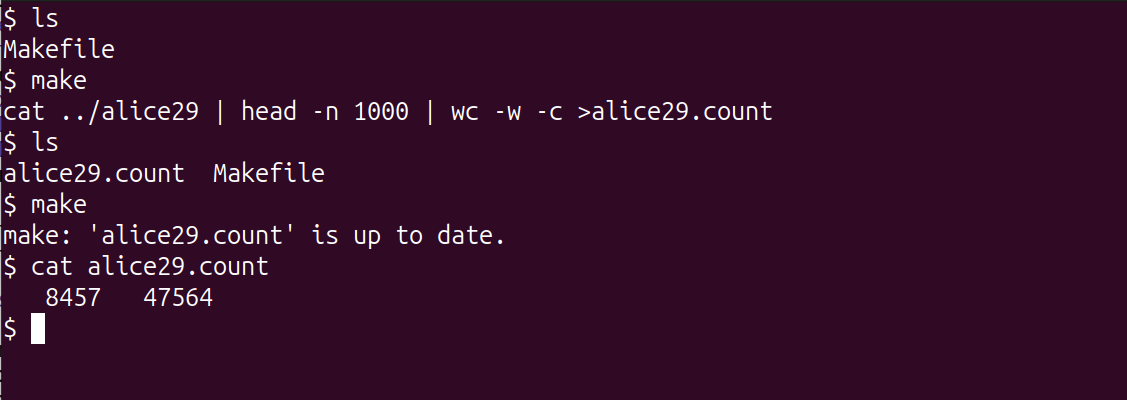
\includegraphics[width=\linewidth]{background/example-v1}
\end{figure}

\end{frame}


%%%%%%%%%%%%%%%%%%%%%%%%%%%%%%%%%%%%%%%%%%%%%%%%%%%
\begin{frame}

\frametitle{``Make'' now}

Make and Makefiles have not disappeared:
\begin{itemize}
  \item The ``make'' program still exists; and to keep something trivial up-to-date, it remains very useful.
\end{itemize}
\vs

Many similar tools have since existed that have ``Make'' in their names:
\begin{itemize}
  \item CMake
  \item qmake
  \item Snakemake
\end{itemize}

\end{frame}


%%%%%%%%%%%%%%%%%%%%%%%%%%%%%%%%%%%%%%%%%%%%%%%%%%%
\begin{frame}

\frametitle{Make}

Their purposes:
\begin{itemize}
  \item CMake -- Cross-platform make, for projects made with C/C++ (for example)
  \item qmake -- Qt projects make, for C++ projects using Qt to make a graphical user interface
  \item Snakemake -- Development of workflows with Python syntax
\end{itemize}

\end{frame}


%%%%%%%%%%%%%%%%%%%%%%%%%%%%%%%%%%%%%%%%%%%%%%%%%%%
\begin{frame}

\frametitle{Snakemake}

So, that is where the ``make'' part of Snake{\green{make}} comes from!
\vs

The ``Snake'' part is due to {\blue{Snake}}make being made with Python and borrows some of Python's syntax.
\vs

But it is a separate program with a different file format.  i.e., Snakemake files are not Python programs.

\end{frame}


%%%%%%%%%%%%%%%%%%%%%%%%%%%%%%%%%%%%%%%%%%%%%%%%%%%%%%%
\begin{frame}

\frametitle{Data sets}

Two sets of text files will be considered.  Both are used to test text compression systems (i.e., my former area of research):
\begin{itemize}
  \item Calgary corpus from the University of Calgary \citep{bcw90:book}.
  \item Canterbury corpus from the University of Canterbury \citep{ab97:dcc}.
\end{itemize}
\vs

While not bioinformatics related, we are all familiar with text and both are publicly available.
\vs

Even so, I have taken only the first 1,024 lines of each since the originals are too large for our purposes.

\end{frame}


